\documentclass[12pt,letterpaper]{article}
\usepackage[T1]{fontenc}
\usepackage[letterpaper,margin=1in]{geometry}
\usepackage{amsmath,amssymb,amsthm,array,booktabs}
\IfFileExists{newtxtext.sty}{\usepackage{newtxtext,newtxmath}}{\usepackage{mathptmx}}
\usepackage{microtype}
\usepackage{tikz}
\usetikzlibrary{arrows.meta,calc}
\usepackage[hidelinks]{hyperref}
\setlength{\parskip}{0.3em}
\setlength{\parindent}{1.2em}
\newtheorem{theorem}{Theorem}[section]
\newtheorem{proposition}[theorem]{Proposition}
\newtheorem{corollary}[theorem]{Corollary}
\newtheorem{lemma}[theorem]{Lemma}
\theoremstyle{definition}
\newtheorem{definition}[theorem]{Definition}
\newtheorem{example}[theorem]{Example}
\theoremstyle{remark}
\newtheorem{remark}[theorem]{Remark}
\numberwithin{equation}{section}
\DeclareMathOperator{\Aut}{Aut}
\DeclareMathOperator{\Ind}{Ind}
\DeclareMathOperator{\Hom}{Hom}
\DeclareMathOperator{\tr}{tr}
\DeclareMathOperator{\Spec}{Spec}
\DeclareMathOperator{\Fix}{Fix}
\DeclareMathOperator{\spanof}{span}
\DeclareMathOperator{\divisor}{div}
\newcommand{\CC}{\mathbb C}
\newcommand{\ZZ}{\mathbb Z}
\newcommand{\RR}{\mathbb R}
\newcommand{\LL}{\mathcal L}
\newcommand{\calO}{\mathcal O}
\newcommand{\bfone}{\mathbf 1}
\title{Representations of finite groups on the Riemann--Roch\\space of a toric variety\\[5pt]
\large Draft 3: Corrected and expanded version}
\author{David Joyner\thanks{Original unpublished manuscript dated June 23, 2002. This is a corrected and expanded draft prepared November 22, 2026.}\thanks{Email: \texttt{wdjoyner@gmail.com}.}}
\date{Original draft: 2002. Corrected and expanded draft: November 2026}
\begin{document}
\maketitle
\begin{abstract}
This AI-aided paper studies finite-group representations on toric Riemann--Roch spaces; details of AI assistance appear in the acknowledgments and a separate revision log. For a finite group of fan automorphisms preserving a torus-invariant Weil divisor on a complete normal toric variety, the Riemann--Roch space is a permutation module on the lattice points of the divisor polytope. We describe its induced-module decomposition and irreducible character multiplicities, and derive a weighted trace formula for finite subgroups of the torus normalizer. For an explicit singular toric surface with involution, we determine the representations associated with every nonnegative multiple of a divisor. We connect these modules with lattice-point graphs, commuting adjacency operators, equivariant Ehrhart counting, graphic zonotopes, and Johnson graphs. For the hypersimplex associated with the edges of a complete graph, we prove that the three Johnson-graph eigenspaces are the three irreducible constituents of the associated symmetric-group representation. The emphasis is on a self-contained synthesis of classical constructions and explicit examples.
\end{abstract}
\tableofcontents

\section{Introduction}
The problem of determining the representation of a finite group $G$ on a Riemann--Roch space $L(D)$ is familiar in the theory of curves. On a toric variety there is an especially accessible approach: torus characters provide a basis of $L(D)$ indexed by lattice points of a polyhedron. A group acting on the fan acts on those lattice points.

This description immediately raises two questions. What are the $G$-submodules generated by the individual lattice-point orbits? And how can one determine the multiplicities of the irreducible constituents of $L(D)$? Each orbit yields an induced permutation module. Its further decomposition is controlled by the character values of $G$ on fixed lattice points, as in Theorem~\ref{thm:orbit} and Corollary~\ref{cor:character}.

The graph-theoretic viewpoint enriches this calculation. A $G$-invariant step set on the character lattice defines a finite graph whose adjacency operator commutes with the representation. Conversely, edge polytopes and graphic zonotopes connect graph automorphisms with toric Riemann--Roch spaces. A particularly concrete instance involves the line graph of $K_n$, which is the Johnson graph $J(n,2)$.

Throughout, irreducible character decompositions are taken over $\CC$, except where an arbitrary field is explicitly allowed. Our running example is a singular complete toric surface with an involution. The surface exhibits both the induced-module calculation and its graph-theoretic refinements.

\section{Related literature}
The two ingredients in our approach are the polytope description of toric global sections and the representation theory of finite permutation actions. Equivariant Ehrhart theory and spectral graph theory place these ingredients in a broader context.

\subsection*{Toric geometry and character theory}
The polytope description of global sections of torus-invariant divisors is standard in toric geometry; see Fulton \cite{Fu93} and Oda \cite{Od88}. Finite-group characters and induction from stabilizers are classical results of representation theory; see Serre \cite{Se77}. Related questions for Riemann--Roch spaces on curves were studied by Joyner and Traves \cite{JT02}. In the toric setting, character monomials make the corresponding group action especially concrete.

\subsection*{Equivariant Ehrhart and spectral graph theory}
Stapledon's 2011 article \cite{St11} systematically develops equivariant Ehrhart theory. Elia, Kim, and Supina \cite{EKS24} explicitly study graphic zonotopes and hypersimplices, among other examples. The spectral theory of Johnson graphs is classical; an overview of related spectral graph theory appears in Brouwer and Haemers \cite{BH12}. The forest-counting formula for graphic zonotopes is established in this literature; see \cite[Section 3.1]{EKS24}. We use these results to connect lattice-point enumeration with toric representations, and give a direct graph-spectral argument for the Johnson-graph example.

For example, the triangle graph has three single-edge forests and three two-edge forests. Its graphic zonotope has Ehrhart polynomial $1+3q+3q^2$. This simple case will reappear in Section~\ref{sec:zonotope}.

\section{Background and notation}\label{sec:background}
We recall the geometry and representation theory underlying the orbit and character formulas. Unless stated otherwise, every toric divisor considered below is invariant under the dense torus.

\subsection{Toric divisors and their lattice points}
Let $N\cong\ZZ^d$ be a lattice, let $M=\Hom_{\ZZ}(N,\ZZ)$, and let $\Delta$ be a complete rational fan in $N_{\RR}$. Write $X=X(\Delta)$ for the associated normal complete toric variety with dense torus $T=\Hom(M,\CC^\times)$. For each ray $\rho\in\Delta(1)$, let $v_\rho\in N$ denote its primitive generator and $D_\rho$ the corresponding torus-invariant prime divisor, namely the \emph{closure} of the orbit $O(\rho)$.

A torus-invariant Weil divisor and its polyhedron are
\begin{equation}\label{eq:polytope}
D=\sum_{\rho\in\Delta(1)} a_\rho D_\rho,
\qquad
P_D=\{u\in M_{\RR}:\langle u,v_\rho\rangle\geq-a_\rho
\text{ for all }\rho\}.
\end{equation}
The sheaf $\calO_X(D)$ is in general reflexive of rank one, not necessarily invertible. Its global sections agree with the Riemann--Roch space
\begin{equation}\label{eq:rr}
L(D)=\{f\in\CC(X)^\times:\divisor(f)+D\geq0\}\cup\{0\}
=\bigoplus_{u\in P_D\cap M}\CC\chi^u.
\end{equation}
The basis theorem is the usual toric character description \cite[Section 3.4]{Fu93}. Completeness makes the set $P_D\cap M$ finite; it may be empty.

\begin{example}\label{ex:p1}
For $X=\mathbb P^1$, let $N=M=\ZZ$ and take the two rays with generators $1$ and $-1$. If $D=aD_++bD_-$, then $P_D=[-a,b]$. When $a+b\geq0$ and $a,b$ are integers, equation~\eqref{eq:rr} has $a+b+1$ character monomials.
\end{example}

\subsection{Group actions and induction}
Let $\Aut(\Delta)\subseteq\operatorname{GL}(N)$ be the lattice automorphisms preserving the fan. The induced action on $M$ is
\begin{equation}\label{eq:dualaction}
(g\cdot u)(v)=u(g^{-1}v).
\end{equation}
If $a_{g\rho}=a_\rho$ for every ray and $g\in G\leq\Aut(\Delta)$, the action preserves both $D$ and $P_D$. On rational functions we use the convention $(g\cdot f)(x)=f(g^{-1}x)$, so
\begin{equation}\label{eq:monomialaction}
g\cdot\chi^u=\chi^{g\cdot u}.
\end{equation}
For $u\in M$, write $G_u=\{g\in G:g\cdot u=u\}$. A permutation module on the orbit $G\cdot u$ is $\CC[G\cdot u]\cong\Ind_{G_u}^G\bfone$.

\begin{example}
If $G=C_2$ interchanges two basis vectors $e_1,e_2$, then $\CC e_1\oplus\CC e_2$ is not irreducible: its invariant line is spanned by $e_1+e_2$ and its sign line by $e_1-e_2$.
\end{example}

\subsection{Notation table}
For reference, the symbols used most frequently are collected below. The running $C_2$ example uses $N=M=\ZZ^2$, with the natural pairing.
\begin{center}
\begin{tabular}{@{}p{0.26\linewidth}p{0.65\linewidth}@{}}
\toprule
$N$, $M$ & Cocharacter lattice and its character dual $N^\vee$.\\
$\Delta$, $X(\Delta)$ & Complete fan and associated normal toric variety.\\
$T$ & Dense algebraic torus of $X(\Delta)$.\\
$D$, $P_D$ & Torus-invariant Weil divisor and its polyhedron.\\
$S_D$ & Finite set $P_D\cap M$ of character exponents.\\
$G_u$ & Stabilizer of $u$ under a finite group $G$.\\
$\rho_D$, $\chi_D$ & Representation on $L(D)$ and its character.\\
$\Gamma_D(B)$, $A$ & Lattice-point graph for step set $B$, and its adjacency matrix.\\
$J(n,2)$ & Johnson graph on the two-element subsets of $\{1,\ldots,n\}$.\\
\bottomrule
\end{tabular}
\end{center}

\section{Orbit modules and character formulas}\label{sec:representation}
The character basis of $L(D)$ is partitioned into finite $G$-orbits. It is natural to ask first for the representation carried by the span of a single orbit and then for the irreducible constituents of the whole space. Induction from stabilizers answers the first question; fixed-point character counts answer the second.

\begin{theorem}[Orbit decomposition]\label{thm:orbit}
Let $X=X(\Delta)$ be a complete normal toric variety over $\CC$. Let $G\leq\Aut(\Delta)$ be finite and let $D=\sum a_\rho D_\rho$ be a $G$-invariant torus-invariant Weil divisor. Put $S_D=P_D\cap M$. Then
\begin{equation}\label{eq:induction}
L(D)\cong\CC[S_D]\cong
\bigoplus_{\mathcal O\in S_D/G}\Ind_{G_u}^G\bfone,
\qquad u\in\mathcal O.
\end{equation}
These are transitive permutation modules. Over $\CC$ they can be decomposed further into irreducible modules. The permutation-module and orbit-sum assertions remain true over any field.
\end{theorem}
\begin{proof}
Equation~\eqref{eq:rr} gives a basis indexed by $S_D$. Since $G$ preserves the rays and coefficients of $D$, the defining inequalities of $P_D$ are carried to one another, so $G$ preserves $S_D$. Equation~\eqref{eq:monomialaction} shows that it permutes the indicated basis without scalar factors. Therefore $L(D)\cong\CC[S_D]$. Each orbit span is a subrepresentation, and choosing a representative $u$ identifies its basis with the coset space $G/G_u$. The standard description of the induced trivial representation proves equation~\eqref{eq:induction}.
\end{proof}

\begin{corollary}[Fixed-point character and multiplicities]\label{cor:character}
Under the hypotheses of Theorem~\ref{thm:orbit}, let $\psi$ be an irreducible complex character of $G$. For every $g\in G$,
\begin{align}
\chi_D(g)&=\tr(\rho_D(g))=\bigl|P_D\cap M^g\bigr|,\label{eq:fixedchar}\\
 m_\psi(D)&=\frac1{|G|}\sum_{g\in G}
 \overline{\psi(g)}\bigl|P_D\cap M^g\bigr|.\label{eq:mult}
\end{align}
Here $M^g=\{u\in M:g\cdot u=u\}$, and $m_\psi(D)$ is the multiplicity of $\psi$ in $L(D)$.
\end{corollary}
\begin{proof}
The matrix of $\rho_D(g)$ in the character basis is a permutation matrix. Its diagonal ones correspond exactly to fixed lattice points. This proves equation~\eqref{eq:fixedchar}. Complex representation theory gives the irreducible character inner product $m_\psi(D)=\langle\chi_D,\psi\rangle_G$, which is equation~\eqref{eq:mult}.
\end{proof}

\begin{remark}
The fixed-point formula gives a character-valued refinement of the lattice-point count when $D$ is dilated, as in equivariant Ehrhart theory \cite{St11,EKS24}. The distinction between orbit modules and irreducible modules is visible already for the action of $C_2$ on two points: the orbit module is the sum of the trivial and sign representations.
\end{remark}

\begin{example}
For a $C_2$-set consisting of seven fixed points and twelve two-point orbits, equation~\eqref{eq:induction} gives $7\bfone+12(\bfone\oplus\operatorname{sgn})=19\bfone\oplus12\operatorname{sgn}$. This is the decomposition occurring in the next section.
\end{example}

\section{A singular toric surface with an involution}\label{sec:surface}
We now study a complete toric surface with three cyclic quotient singularities and an involution that interchanges two rays. The geometry is simple enough to compute the Riemann--Roch character and its irreducible decomposition for every nonnegative multiple of a divisor.

Put $N=\ZZ^2$ and choose primitive rays
\begin{equation}\label{eq:rays}
v_1=(2,-1),\quad v_2=(-1,2),\quad v_3=(-1,-1).
\end{equation}
Take the maximal cones $\sigma_1=\operatorname{Cone}(v_1,v_2)$,
$\sigma_2=\operatorname{Cone}(v_2,v_3)$, and
$\sigma_3=\operatorname{Cone}(v_3,v_1)$, together with their faces. This is a complete fan: $v_1+v_2+v_3=0$ and each consecutive determinant is $3$. Each affine chart has a cyclic $A_2$ singularity over $\CC$.

\begin{figure}[ht]
\centering
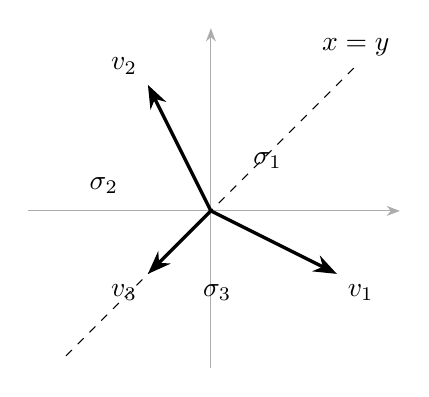
\begin{tikzpicture}[scale=0.80,>=Stealth]
\draw[->,gray!65] (-2.9,0)--(3.0,0);
\draw[->,gray!65] (0,-2.5)--(0,2.9);
\draw[very thick,->] (0,0)--(2,-1) node[below right] {$v_1$};
\draw[very thick,->] (0,0)--(-1,2) node[above left] {$v_2$};
\draw[very thick,->] (0,0)--(-1,-1) node[below left] {$v_3$};
\node at (0.9,0.8) {$\sigma_1$};
\node at (-1.7,0.4) {$\sigma_2$};
\node at (0.1,-1.3) {$\sigma_3$};
\draw[dashed] (-2.3,-2.3)--(2.3,2.3) node[above] {$x=y$};
\end{tikzpicture}
\caption{A complete three-cone fan with its involution axis. The cones have lattice index three and the surface is singular.}\label{fig:fan}
\end{figure}

Write $\rho_i=\RR_{\geq0}v_i$ and $D_i=V(\rho_i)$ for the invariant divisors. A direct support-function calculation shows that $D=\sum d_iD_i$ is Cartier exactly when $d_1\equiv d_2\equiv d_3\pmod3$. The affine coordinate rings are
\begin{equation}\label{eq:charts}
\begin{aligned}
\CC[U_{\sigma_1}]&\cong\CC[x_1,x_2,x_3]/(x_1^3-x_2x_3),\\
\CC[U_{\sigma_2}]&\cong\CC[y_1,y_2,y_3]/(y_2^3-y_1y_3),\\
\CC[U_{\sigma_3}]&\cong\CC[z_1,z_2,z_3]/(z_2^3-z_1z_3).
\end{aligned}
\end{equation}
For example, the three exponents on $U_{\sigma_2}$ are $(-2,-1)$, $(-1,0)$, and $(-1,1)$; their relation is $3(-1,0)=(-2,-1)+(-1,1)$. Similarly, the exponents on $U_{\sigma_1}$ are $(1,1)$, $(1,2)$, and $(2,1)$, and on $U_{\sigma_3}$ they are $(0,-1)$, $(-1,-2)$, and $(1,-1)$. The swap $g(x,y)=(y,x)$ exchanges $v_1$ and $v_2$, fixes $v_3$, fixes $U_{\sigma_1}$, and exchanges $U_{\sigma_2}$ and $U_{\sigma_3}$.

Let $G=\langle g\rangle\cong C_2$ and choose
\begin{equation}\label{eq:Dsurface}
D=6D_1+6D_2,
\qquad
P_D=\{(x,y):2x-y\geq-6,\ -x+2y\geq-6,\ x+y\leq0\}.
\end{equation}
Its vertices are $(-6,-6),(-2,2),(2,-2)$, and it is $G$-invariant.

\begin{proposition}\label{prop:cyclic}
For every integer $q\geq0$,
\begin{align}
\dim L(qD)&=24q^2+6q+1,\label{eq:ehrhartsurf}\\
\tr\bigl(g\mid L(qD)\bigr)&=6q+1,\label{eq:fixedsurf}\\
L(qD)&\cong(12q^2+6q+1)\bfone\oplus
12q^2\operatorname{sgn}.\label{eq:repsurf}
\end{align}
\end{proposition}
\begin{proof}
The triangle $P_D$ has Euclidean area $24$. Its three edges have primitive lattice lengths $4$, $4$, and $4$, respectively. Pick's theorem gives $|qP_D\cap\ZZ^2|=24q^2+6q+1$ for every $q\geq1$, and the same expression equals $1$ at $q=0$. The fixed points under $g$ lie on $x=y$. In $qP_D$ these are precisely $(a,a)$ for $-6q\leq a\leq0$, giving $6q+1$ points. The two characters of $C_2$ have multiplicities $(\dim\pm\tr(g))/2$. Substitution yields equation~\eqref{eq:repsurf}.
\end{proof}

\begin{example}
At $q=1$ there are $31$ lattice points, seven fixed points, and twelve two-element orbits. Accordingly $L(D)=19\bfone\oplus12\operatorname{sgn}$. This illustrates how the orbit decomposition leads to explicit irreducible multiplicities.
\end{example}

\section{Lattice-point graphs and commuting operators}\label{sec:graphs}
A graph structure on $P_D\cap M$ gives a second operator on the same Riemann--Roch space. The resulting spectral decomposition is particularly useful when the graph and its group action are sufficiently symmetric.

\begin{definition}\label{def:latticegraph}
Assume the hypotheses of Theorem~\ref{thm:orbit}. Let $B\subset M\setminus\{0\}$ be finite with $B=-B$ and $gB=B$ for every $g\in G$. The \emph{lattice-point graph} $\Gamma_D(B)$ has vertex set $S_D$; distinct vertices $u,v$ are adjacent exactly when $u-v\in B$. Let $A$ denote its adjacency operator on $\CC[S_D]$.
\end{definition}

\begin{theorem}[Commuting adjacency theorem]\label{thm:commute}
For $G$, $D$, and $B$ as in Definition~\ref{def:latticegraph}, every $g\in G$ is an automorphism of $\Gamma_D(B)$, and
\begin{equation}\label{eq:commute}
A\rho_D(g)=\rho_D(g)A.
\end{equation}
Consequently, every adjacency eigenspace is a $G$-subrepresentation. More precisely, over $\CC$ there is a decomposition
\begin{equation}\label{eq:spectral}
L(D)=\bigoplus_{\lambda\in\Spec(A)}\ \bigoplus_{\psi\in\widehat G}E_{\lambda,\psi},
\end{equation}
where $E_{\lambda,\psi}$ is the $\psi$-isotypic component of the $\lambda$-eigenspace. Some components can be zero.
\end{theorem}
\begin{proof}
If $u-v\in B$, then $g(u)-g(v)=g(u-v)\in B$, so $g$ preserves edges. For a vertex basis vector $e_u$, the vector $Ae_u$ is the sum of its neighbors. Applying $g$ takes this sum to the neighbors of $g(u)$, which is $A\rho_D(g)e_u$. Thus equation~\eqref{eq:commute} holds on a basis. The adjacency matrix of an undirected finite graph is real symmetric, so it is diagonalizable over $\CC$. Its eigenspaces are $G$-stable by commutation and completely reducible as complex $G$-modules. This proves equation~\eqref{eq:spectral}.
\end{proof}

\begin{proposition}[Twisted walk trace]\label{prop:walks}
For every integer $r\geq0$ and $g\in G$,
\begin{equation}\label{eq:walks}
\tr\bigl(\rho_D(g)A^r\bigr)=
\sum_{u\in S_D}(A^r)_{u,g(u)}.
\end{equation}
Thus the right-hand side counts ordered graph walks of length $r$ from a vertex to its $g$-translate, summed over all starting vertices. At $r=0$ it recovers the fixed-point character formula.
\end{proposition}
\begin{proof}
The entries $(A^r)_{u,v}$ count walks of length $r$ from $u$ to $v$. In the basis indexed by $S_D$, the diagonal coefficient of $\rho_D(g)A^r$ at $e_u$ is $(A^r)_{g^{-1}u,u}$. Reindexing by $g^{-1}u$ gives the right-hand side of equation~\eqref{eq:walks}.
\end{proof}

\begin{example}[The graph on the triangle]\label{ex:graph31}
For the divisor of Section~\ref{sec:surface}, choose
\[
B=\{(a,b)\in\{-1,0,1\}^2:(a,b)\ne(0,0)\}.
\]
This is the eight-neighbor lattice graph and $B$ is invariant under coordinate swap. Its $31$ vertices form a connected graph with $85$ undirected edges. Under the involution its $31$-dimensional vertex space splits as an invariant adjacency block of dimension $19$ and an anti-invariant block of dimension $12$. Five edges are exchanged endpoint-by-endpoint by $g$, so equation~\eqref{eq:walks} gives $\tr(\rho_D(g)A)=10$. The edge count and last trace were independently checked by exhaustive integer enumeration in \texttt{verify\_examples.py}; no numerical eigenvalue approximation is used in the proof.
\end{example}

\begin{remark}
The adjacency spectrum depends on the chosen step set $B$; it is not an invariant of $D$ alone. Conversely, commutation need not imply that each eigenspace is irreducible. The Johnson graph in Section~\ref{sec:johnson} is a case where an especially symmetric adjacency operator does resolve all constituents.
\end{remark}

\section{From a graph to a toric polytope}\label{sec:zonotope}
We next reverse the direction: start with a graph and construct a polytope whose lattice-point representation is a toric Riemann--Roch space. Graphic zonotopes display the role of spanning forests particularly clearly.

\begin{definition}
Let $H$ be a connected simple graph on vertices $\{1,\ldots,n\}$. Its \emph{graphic zonotope} is
\begin{equation}\label{eq:zonotope}
Z_H=\sum_{\{i,j\}\in E(H)}[e_i,e_j]\subset\RR^n,
\end{equation}
with the sum interpreted as a Minkowski sum. It lies in the affine lattice hyperplane $\sum_i x_i=|E(H)|$, with difference lattice $\{x\in\ZZ^n:\sum_i x_i=0\}$. The graph automorphism group acts by coordinate permutations and preserves $Z_H$.
\end{definition}

\begin{proposition}[Classical graphic-zonotope enumeration]\label{prop:forests}
For every connected simple graph $H$ and $q\geq0$,
\begin{equation}\label{eq:forest}
|qZ_H\cap\ZZ^n|=
\sum_{\substack{F\subseteq E(H)\\F\text{ is a forest}}}q^{|F|}.
\end{equation}
Consequently, if $\LL_H$ denotes the ample line bundle on the projective toric variety of $Z_H$, then $\dim H^0(X_H,\LL_H^{\otimes q})$ is the forest enumerator in equation~\eqref{eq:forest}. The formula is classical; see \cite[Section 3.1]{EKS24}.
\end{proposition}
\begin{proof}
Orient the edges arbitrarily. Translating $Z_H$ by a lattice vector gives the zonotope generated by incidence vectors $e_i-e_j$. A subset of these vectors is linearly independent exactly when the corresponding edges form a forest. The incidence matrix of a graph is totally unimodular. Consequently every independent family generates a saturated sublattice of its span, and each such family has normalized lattice index one. The standard half-open parallelotope decomposition of a lattice zonotope therefore contributes $q^{|F|}$ lattice points from each independent family $F$, proving the formula. The identification with global sections is the character-basis theorem applied to the lattice polytope $Z_H$, with the affine lattice and its natural line-bundle linearization understood.
\end{proof}

\begin{example}[The triangle graph]\label{ex:K3}
For $H=K_3$, the graphic zonotope is a hexagon. After translation by $(1,1,1)$ it is
\[
P=\operatorname{conv}\{\text{permutations of }(-1,0,1)\}
\subset\{x_1+x_2+x_3=0\}.
\]
The three single-edge forests, the three two-edge forests, and the empty forest give
\begin{equation}\label{eq:k3poly}
|qP\cap M|=1+3q+3q^2.
\end{equation}
The coordinate-permutation action of $S_3$ on this hexagon has character values
\begin{equation}\label{eq:K3chars}
\chi_q(1)=3q^2+3q+1,\quad
\chi_q((12))=2\lfloor q/2\rfloor+1,\quad
\chi_q((123))=1.
\end{equation}
Indeed, the hexagon is the intersection of the plane $x_1+x_2+x_3=0$ with the inequalities $|x_i|\leq1$. For a transposition-fixed lattice point of $qP$, write $x_1=x_2=a$ and $x_3=-2a$; thus $|a|\leq q/2$. A point fixed by a $3$-cycle has all three coordinates equal, so only the origin survives. Taking inner products with the characters of $S_3$ yields
\begin{equation}\label{eq:k3reps}
\begin{split}
H^0(X_{K_3},\LL_{K_3}^{\otimes q})\cong{}&
\Bigl(\frac{q(q+1)}2+\lfloor q/2\rfloor+1\Bigr)\bfone\\
&\oplus\Bigl(\frac{q(q+1)}2-\lfloor q/2\rfloor\Bigr)\operatorname{sgn}\\
&\oplus q(q+1)V_{\mathrm{std}}.
\end{split}
\end{equation}
At $q=1$ the seven lattice points comprise a regular $S_3$-orbit and the origin, giving $2\bfone\oplus\operatorname{sgn}\oplus2V_{\mathrm{std}}$.
\end{example}

\section{Hypersimplices, line graphs, and irreducible constituents}\label{sec:johnson}
The next family makes the graph-spectrum connection particularly precise. The adjacency operator of a Johnson graph separates all the irreducible pieces of the corresponding toric Riemann--Roch representation.

Let $n\geq4$. The \emph{second hypersimplex} is
\begin{equation}\label{eq:hypersimplex}
\Delta(2,n)=\operatorname{conv}\{e_i+e_j:1\leq i<j\leq n\}
=\{x\in[0,1]^n:\sum_i x_i=2\}.
\end{equation}
Its lattice points are exactly the $\binom n2$ edge vectors of $K_n$. The normal fan yields a projective toric variety $X_n$ with an ample, $S_n$-linearized line bundle $\LL_n$. For clarity, the linearization can be obtained from the monomial projective embedding associated to the hypersimplex, on whose homogeneous coordinates $S_n$ acts by permuting the labels $\{i,j\}$. In particular,
\begin{equation}\label{eq:edgeaction}
H^0(X_n,\LL_n)\cong\CC[E(K_n)]
\end{equation}
with its untwisted edge-permutation action.

The \emph{Johnson graph} $J(n,2)$ has vertex set $E(K_n)$, two edges being adjacent if they have exactly one endpoint in common. Equivalently, it is the line graph of $K_n$.

\begin{figure}[ht]
\centering
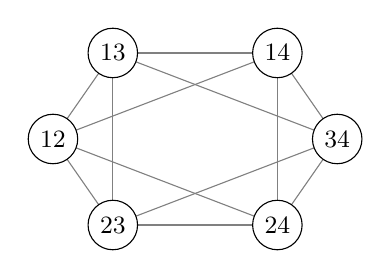
\begin{tikzpicture}[scale=0.95,every node/.style={draw,circle,fill=white,inner sep=2.5pt,font=\small}]
\coordinate (L) at (-1.9,0); \coordinate (R) at (1.9,0);
\coordinate (TL) at (-1.1,1.15); \coordinate (TR) at (1.1,1.15);
\coordinate (BR) at (1.1,-1.15); \coordinate (BL) at (-1.1,-1.15);
\draw[gray] (TL)--(TR)--(BR)--(BL)--cycle;
\foreach \v in {TL,TR,BR,BL}{\draw[gray] (L)--(\v); \draw[gray] (R)--(\v);}
\node at (L) {$12$}; \node at (R) {$34$};
\node at (TL) {$13$}; \node at (TR) {$14$};
\node at (BR) {$24$}; \node at (BL) {$23$};
\end{tikzpicture}
\caption{The Johnson graph $J(4,2)$, isomorphic to the octahedral graph. Labels denote the edges of $K_4$. The two opposite vertices $12$ and $34$ are not adjacent.}\label{fig:johnson}
\end{figure}

\begin{theorem}[Johnson spectral decomposition]\label{thm:johnson}
For every $n\geq4$, the adjacency operator $A$ of $J(n,2)$ on $H^0(X_n,\LL_n)$ has exactly three eigenvalues and multiplicities:
\begin{equation}\label{eq:johnsoneigs}
\begin{array}{c|ccc}
\lambda&2(n-2)&n-4&-2\\\hline
\dim E_\lambda&1&n-1&\dfrac{n(n-3)}2.
\end{array}
\end{equation}
Each eigenspace is an irreducible $S_n$-module. In characteristic zero,
\begin{equation}\label{eq:specht}
H^0(X_n,\LL_n)\cong
S^{(n)}\oplus S^{(n-1,1)}\oplus S^{(n-2,2)},
\end{equation}
with the three constituents occurring in the displayed eigenvalue order.
\end{theorem}
\begin{proof}
Let $r=\binom n2$ and form the $n\times r$ unsigned vertex-edge incidence matrix $R$ of $K_n$. Each column has two ones. Distinct edge columns have scalar product one if their edges meet and zero otherwise. Therefore
\begin{equation}\label{eq:Rrelations}
R^{\mathsf T}R=A+2I_r,
\qquad
RR^{\mathsf T}=(n-2)I_n+J_n,
\end{equation}
where $J_n$ is the all-ones matrix. The second matrix has eigenvalue $2(n-1)$ on the constant vector and $n-2$ on its orthogonal complement. Since $n\geq4$, $R$ has rank $n$. The nonzero eigenvalues of $R^{\mathsf T}R$ are those of $RR^{\mathsf T}$ with the same multiplicities. Subtracting two proves the eigenvalues and multiplicities in equation~\eqref{eq:johnsoneigs}; the remaining $r-n=n(n-3)/2$ eigenvectors lie in $\ker R$.

The action of $S_n$ on unordered pairs has exactly three orbits on \emph{ordered pairs} of unordered pairs: equal, meeting in one vertex, and disjoint. Hence the algebra of endomorphisms commuting with $S_n$ on $\CC[E(K_n)]$ has dimension three: a commuting matrix must be constant on each such orbit. Since complex representations are semisimple, its dimension is the sum of squares of irreducible multiplicities. The existence of the three distinct nonzero $S_n$-stable eigenspaces already found forces each eigenspace to be irreducible and pairwise nonisomorphic. The constant eigenspace is $S^{(n)}$; the image under $R^{\mathsf T}$ of the zero-sum coordinate subspace of $\CC^n$ is the standard module $S^{(n-1,1)}$. The remaining constituent is $S^{(n-2,2)}$, as follows also from the standard decomposition of the two-subset permutation module (Young's rule; see \cite{Se77} for the representation-theoretic framework).
\end{proof}

\begin{example}\label{ex:n4}
When $n=4$, the Johnson graph is an octahedral graph (Figure~\ref{fig:johnson}). Its adjacency eigenvalues are $4,0,-2$ of multiplicities $1,3,2$. Thus the six-dimensional Riemann--Roch representation is $S^{(4)}\oplus S^{(3,1)}\oplus S^{(2,2)}$, with graph eigenspaces furnishing the irreducible decomposition directly.
\end{example}

\begin{remark}
Theorem~\ref{thm:johnson} combines classical properties of hypersimplices, two-subset permutation modules, and Johnson-graph spectra. What is useful here is that the adjacency eigenspaces identify the irreducible constituents of a toric Riemann--Roch representation without computing its full character table.
\end{remark}

\section{Beyond pure permutation actions: the torus normalizer}\label{sec:normalizer}
A natural generalization arises when an automorphism of $X$ also translates the dense torus. Fan automorphisms permute the character monomials, but a torus translation scales them. What becomes of the fixed-point character formula for a finite subgroup of the torus normalizer? The appropriate answer is a weighted trace, with one scalar weight for each fixed lattice exponent.

Consider a finite subgroup of the semidirect product $T\rtimes\Aut(\Delta)$ that preserves the coefficients of $D$ under its fan-automorphism projection. Write an element as $h=t\circ a$, with $t\in T$ and $a\in\Aut(\Delta)$. Let $a_M$ denote the contragredient action on $M$ from equation~\eqref{eq:dualaction}. With the pullback convention of Section~\ref{sec:background},
\begin{equation}\label{eq:normalizer}
h\cdot\chi^u=\chi^{a_Mu}(t^{-1})\chi^{a_Mu}.
\end{equation}
Thus the character basis is permuted \emph{up to scalar}; this is a monomial representation rather than generally a permutation module.

\begin{proposition}[Weighted fixed-point trace]\label{prop:weighted}
For such an element $h=t\circ a$,
\begin{equation}\label{eq:weighted}
\tr(h\mid L(D))=\sum_{\substack{u\in P_D\cap M\\a_Mu=u}}
\chi^u(t^{-1}).
\end{equation}
\end{proposition}
\begin{proof}
In equation~\eqref{eq:normalizer}, the $u$th diagonal coefficient vanishes unless $a_Mu=u$, in which case it is $\chi^u(t^{-1})$. Summing the diagonal coefficients proves the formula.
\end{proof}

\begin{example}
On $\mathbb P^1$ with the usual torus $\CC^\times$, consider $D=D_+$ and $P_D=\{-1,0\}$ in the convention of Example~\ref{ex:p1}. A torsion point $t\in T$ fixes both lattice exponents but has trace $\chi^{-1}(t^{-1})+1=t+1$, not necessarily $2$. Hence counting fixed lattice points would give the wrong trace for torus translations.
\end{example}

\section{Summary and open questions}\label{sec:summary}
The orbit theorem, its character formula, and the weighted normalizer formula describe permutation and monomial actions on toric section spaces. The singular surface example provides explicit formulas for every $L(qD)$. The lattice-point graph construction adds commuting adjacency operators and twisted-walk traces. Graphic zonotopes connect toric section dimensions with forest enumeration, and the Johnson graph realizes a complete irreducible decomposition by adjacency eigenspaces.

The following questions describe possible further work, not established results. First, for which naturally selected $G$-invariant graphs on $P_D\cap M$ do adjacency eigenspaces separate all irreducible constituents? Second, can additional canonical operators distinguish multiplicities when one adjacency matrix cannot? Third, to what extent does the sequence of representation classes $[L(qD)]$, for all $q\geq0$, determine the $G$-equivariant divisor class? Without extra assumptions the inverse problem fails even for trivial $G$: on $\mathbb P^1\times\mathbb P^1$, the non-linearly-equivalent divisors of bidegrees $(1,5)$ and $(2,3)$ both have twelve global sections. The problem becomes interesting only after specifying what information and hypotheses are retained.

\section{Glossary}
This glossary supplies brief reminders of terminology introduced in the background; it is not a substitute for the statements and proofs.
\begin{description}
\item[Adjacency operator.] The linear operator sending each vertex basis vector to the sum of its neighbors.
\item[Character lattice.] The lattice $M$ of algebraic characters of the dense torus.
\item[Equivariant Ehrhart counting.] Counting lattice points in dilated polytopes while retaining their permutation characters under a symmetry group.
\item[Fan automorphism.] A lattice automorphism preserving every cone of a fan as a collection.
\item[Graphic zonotope.] The Minkowski sum of edge segments of a finite graph.
\item[Hypersimplex.] The convex hull of zero-one vectors of prescribed coordinate sum.
\item[Induced permutation module.] The representation $\Ind_H^G\bfone\cong\CC[G/H]$.
\item[Johnson graph.] The graph on subsets of fixed cardinality, with adjacency determined by intersection size.
\item[Reflexive divisor sheaf.] The rank-one coherent sheaf $\calO_X(D)$ associated to a Weil divisor on a normal variety; it need not be locally free.
\item[Toric linearization.] A compatible action on a line bundle lifting an action on the base variety.
\item[Twisted-walk trace.] The trace $\tr(\rho(g)A^r)$, which counts length-$r$ walks from $u$ to $g(u)$.
\end{description}

\section*{Acknowledgments}
This paper benefited from an AI-assisted mathematical review by Carbon (Claude) and from mathematical exposition, independent calculations, graph-theoretic development, verification scripts, and editorial assistance by ChatGPT (OpenAI, GPT-6) in November 2026. AI review is not an independent certification of correctness. The separate revision log records the historical changes, verification levels, and limitations of source checking.

\begin{thebibliography}{99}
\bibitem[BH12]{BH12} A. E. Brouwer and W. H. Haemers, \emph{Spectra of Graphs}, Universitext, Springer, New York, 2012.
\bibitem[EKS24]{EKS24} S. Elia, D. Kim, and M. Supina, Techniques in equivariant Ehrhart theory, \emph{Ann. Comb.} \textbf{28} (2024), 819--870, doi:10.1007/s00026-023-00673-z.
\bibitem[Fu93]{Fu93} W. Fulton, \emph{Introduction to Toric Varieties}, Annals of Mathematics Studies 131, Princeton University Press, Princeton, NJ, 1993.
\bibitem[Ja78]{Ja78} G. D. James, \emph{The Representation Theory of the Symmetric Groups}, Lecture Notes in Mathematics 682, Springer, Berlin, 1978.
\bibitem[JT02]{JT02} D. Joyner and W. Traves, Representations of finite groups on Riemann--Roch spaces, preprint (2002), arXiv:math/0210408.
\bibitem[Od88]{Od88} T. Oda, \emph{Convex Bodies and Algebraic Geometry: An Introduction to the Theory of Toric Varieties}, Springer, Berlin, 1988.
\bibitem[Se77]{Se77} J.-P. Serre, \emph{Linear Representations of Finite Groups}, Springer, New York, 1977.
\bibitem[St11]{St11} A. Stapledon, Equivariant Ehrhart theory, \emph{Adv. Math.} \textbf{226} (2011), 3622--3654.
\end{thebibliography}
\end{document}
